
% This LaTeX was auto-generated from MATLAB code.
% To make changes, update the MATLAB code and republish this document.

\documentclass{article}
\usepackage{graphicx}
\usepackage{color}

    \sloppy
    \definecolor{lightgray}{gray}{0.5}
    \setlength{\parindent}{0pt}

    \begin{document}


        \begin{verbatim}
    clear all; close all; clc
    load learjet24_lin.mat

    t_step = 0.1;
    A	= expm(A_long * t_step);
    B	= ( A_long \ (A - eye(4)) )*B_long ;
    C = eye(4);
    D = [0];
    Q	= 0.01*eye(4);
    R	= 0.1*eye(2);

    V	= diag([5 1 0.1 0.1])
    W	= diag([5 1 0.1 0.1])
    G = eye(4);
    H = [0];

    sys = ss(A,B,C,D)
    sysKalman = ss(A,[B G],C,[])

    [K,S,E] = dlqr(A,B,Q,R);

    sys2 = kalman(sysKalman ,V,W,[]);

    F = lqgreg(sysKalman,K);

    clsys = feedback(sys,F,+1);
    step(sysKalman,'r--',clsys,'b-',10)
    \end{verbatim}

            \color{lightgray} \begin{verbatim}
    V =

        5.0000         0         0         0
             0    1.0000         0         0
             0         0    0.1000         0
             0         0         0    0.1000


    W =

        5.0000         0         0         0
             0    1.0000         0         0
             0         0    0.1000         0
             0         0         0    0.1000


    sys =

      A = 
                   x1          x2          x3          x4
       x1       0.998    0.001249     -0.1139      -3.217
       x2     -0.0192      0.9031       60.32     0.03315
       x3   0.0001033  -0.0009437       0.844  -0.0001647
       x4   5.114e-06  -4.909e-05     0.09256           1

      B = 
                   u1          u2
       x1     0.05285    -0.02295
       x2      -48.36     -0.1087
       x3      -1.325   -0.003216
       x4    -0.06816  -0.0001653

      C = 
           x1  x2  x3  x4
       y1   1   0   0   0
       y2   0   1   0   0
       y3   0   0   1   0
       y4   0   0   0   1

      D = 
           u1  u2
       y1   0   0
       y2   0   0
       y3   0   0
       y4   0   0

    Continuous-time state-space model.


    sysKalman =

      A = 
                   x1          x2          x3          x4
       x1       0.998    0.001249     -0.1139      -3.217
       x2     -0.0192      0.9031       60.32     0.03315
       x3   0.0001033  -0.0009437       0.844  -0.0001647
       x4   5.114e-06  -4.909e-05     0.09256           1

      B = 
                   u1          u2          u3          u4          u5          u6
       x1     0.05285    -0.02295           1           0           0           0
       x2      -48.36     -0.1087           0           1           0           0
       x3      -1.325   -0.003216           0           0           1           0
       x4    -0.06816  -0.0001653           0           0           0           1

      C = 
           x1  x2  x3  x4
       y1   1   0   0   0
       y2   0   1   0   0
       y3   0   0   1   0
       y4   0   0   0   1

      D = 
           u1  u2  u3  u4  u5  u6
       y1   0   0   0   0   0   0
       y2   0   0   0   0   0   0
       y3   0   0   0   0   0   0
       y4   0   0   0   0   0   0

    Continuous-time state-space model.

    \end{verbatim} \color{black}
    
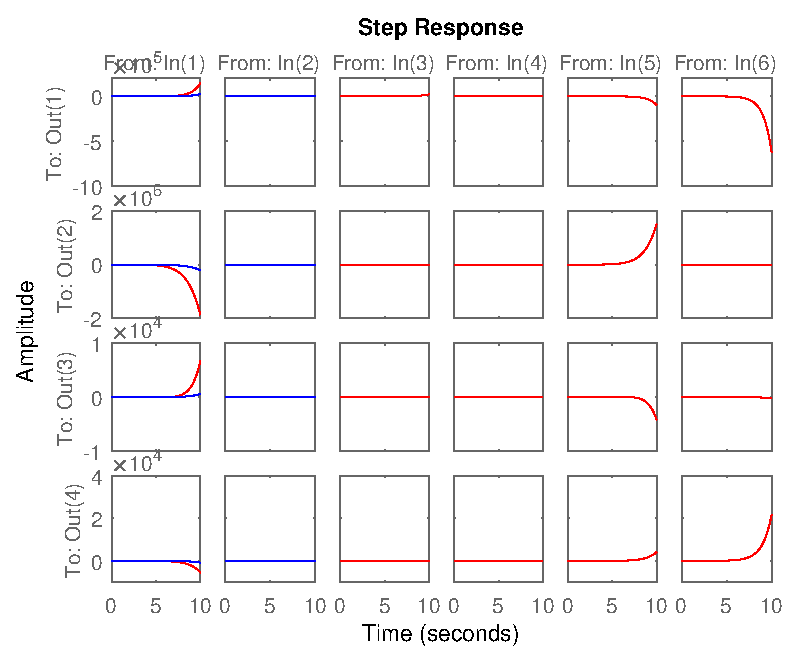
\includegraphics [width=4in]{hw4_p3_01.eps}



\end{document}
    
